 \documentclass{beamer}
\mode<presentation>
\usepackage{amsmath}
\usepackage{amssymb}
%\usepackage{advdate}
\usepackage{graphicx}
\usepackage{adjustbox}
\usepackage{subcaption}
\usepackage{enumitem}
\usepackage{multicol}
\usepackage{mathtools}
\usepackage{listings}
\usepackage{url}
\def\UrlBreaks{\do\/\do-}
\usetheme{Boadilla}
\usecolortheme{lily}
\let\vec\mathbf
\setbeamertemplate{footline}
{
  \leavevmode%
  \hbox{%
  \begin{beamercolorbox}[wd=\paperwidth,ht=2.25ex,dp=1ex,right]{author in head/foot}%
    \insertframenumber{} / \inserttotalframenumber\hspace*{2ex} 
  \end{beamercolorbox}}%
  \vskip0pt%
}
\setbeamertemplate{navigation symbols}{}

\providecommand{\nCr}[2]{\,^{#1}C_{#2}} % nCr
\providecommand{\nPr}[2]{\,^{#1}P_{#2}} % nPr
\providecommand{\mbf}{\mathbf}
\providecommand{\pr}[1]{\ensuremath{\Pr\left(#1\right)}}
\providecommand{\qfunc}[1]{\ensuremath{Q\left(#1\right)}}
\providecommand{\sbrak}[1]{\ensuremath{{}\left[#1\right]}}
\providecommand{\lsbrak}[1]{\ensuremath{{}\left[#1\right.}}
\providecommand{\rsbrak}[1]{\ensuremath{{}\left.#1\right]}}
\providecommand{\brak}[1]{\ensuremath{\left(#1\right)}}
\providecommand{\lbrak}[1]{\ensuremath{\left(#1\right.}}
\providecommand{\rbrak}[1]{\ensuremath{\left.#1\right)}}
\providecommand{\cbrak}[1]{\ensuremath{\left\{#1\right\}}}
\providecommand{\lcbrak}[1]{\ensuremath{\left\{#1\right.}}
\providecommand{\rcbrak}[1]{\ensuremath{\left.#1\right\}}}
\theoremstyle{remark}
\newtheorem{rem}{Remark}
\newcommand{\sgn}{\mathop{\mathrm{sgn}}}
\providecommand{\abs}[1]{\vert#1\vert}
\providecommand{\res}[1]{\Res\displaylimits_{#1}} 
\providecommand{\norm}[1]{\lVert#1\rVert}
\providecommand{\mtx}[1]{\mathbf{#1}}
\providecommand{\mean}[1]{E[ #1 ]}
\providecommand{\fourier}{\overset{\mathcal{F}}{ \rightleftharpoons}}
%\providecommand{\hilbert}{\overset{\mathcal{H}}{ \rightleftharpoons}}
\providecommand{\system}[1]{\overset{\mathcal{#1}}{ \longleftrightarrow}}
%\providecommand{\system}{\overset{\mathcal{H}}{ \longleftrightarrow}}
	%\newcommand{\solution}[2]{\vec{Solution:}{#1}}
%\newcommand{\solution}{\noindent \vec{Solution: }}
\providecommand{\dec}[2]{\ensuremath{\overset{#1}{\underset{#2}{\gtrless}}}}
\newcommand{\myvec}[1]{\ensuremath{\begin{pmatrix}#1\end{pmatrix}}}


\lstset{
%language=C,
frame=single, 
breaklines=true,
columns=fullflexible
}
\lstset{
  language=C,
  basicstyle=\ttfamily\footnotesize,
  keywordstyle=\color{blue}\bfseries,
  commentstyle=\color{gray}\itshape,
  stringstyle=\color{orange},
  numbers=left,
  numberstyle=\tiny\color{gray},
  breaklines=true,
  frame=single,
  showstringspaces=false,
  tabsize=4,
  captionpos=b
}
\numberwithin{equation}{section}
\lstset{
  language=Python,
  basicstyle=\ttfamily\small,
  keywordstyle=\color{blue},
  stringstyle=\color{orange},
  numbers=left,
  numberstyle=\tiny\color{gray},
  breaklines=true,
  showstringspaces=false
}

\title{Problem 4.8.31}
\author{Sujal Rajani}

\date{\today} 
\begin{document}

\begin{frame}
\titlepage
\end{frame}

\section{Question}
\begin{frame}{Question}
\textbf{QUESTION}
\\
 Given $\vec{a}$=2$\hat{i}$ -$\hat{j}$+ $\hat{k}$, $\vec{b}$=3$\hat{i}$-$\hat{k}$ and $\vec{c}$=2$\hat{i}$+$\hat{j}$-2 $\hat{k}$ Find a vector  $\vec{d}$ which is perpendicular to both $\vec{a}$ and $\vec{b}$and $\vec{c}$.$\vec{d}$=3.
\end{frame}
\begin{frame}{Solution}
\textbf{SOLUTION}
as mention in the question :
\begin{align*}
\vec{a}=\myvec{2\\-1\\1},\vec{b}=\myvec{3\\0\\-1},\vec{c}=\myvec{2\\1\\-2}
\end{align*}
\begin{equation}
    \vec{a}^\top\vec{d}=0, \vec{b}^\top\vec{d}=0,  \vec{c}^\top\vec{d}=3.
\end{equation}
\begin{align*}
    \myvec{\vec{a}&\vec{b}}^\top\vec{d}=\myvec{0\\0}
    \\
    \myvec{2&-1&1\\3&0&-1}\vec{d}=\myvec{0\\0}.
    \\
    \vec{d}=k\myvec{1\\5\\3}
\end{align*}
 \end{frame}
\begin{frame}{Solution}
k is a constant 
\\
by equation (1.1):
\begin{align*}
\vec{c}^\top\vec{d}=3
\\
    \myvec{2\\1\\-2}^\top\vec{d}=3
    \\
    k=\dfrac{3}{1}.
\end{align*}
the position vector $\vec{d}$:
\begin{align*}
    \vec{d}=\myvec{3\\15\\9}
\end{align*}
     \end{frame}
       \begin{frame}[fragile]
    \begin{figure}[H]
    \centering
    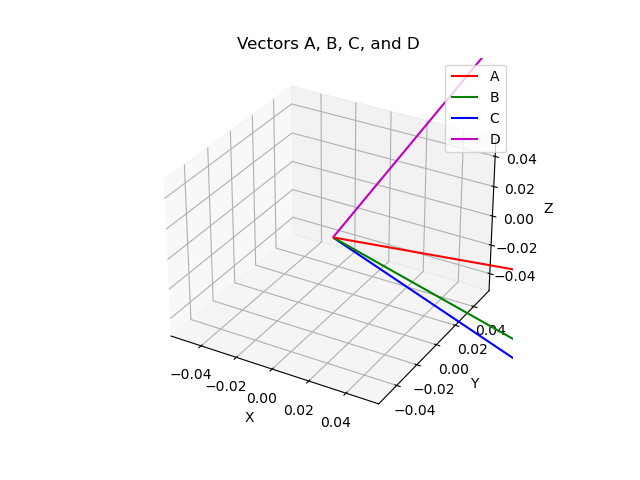
\includegraphics[width = 0.6\columnwidth]{../figs/img.png}
    \caption*{}
    \label{figs}
\end{figure}
\end{frame}
\section{ C Code}
\begin{frame}[fragile]
\frametitle{C Code }
\begin{lstlisting}[language=C]
#include <stdio.h>

int main() {
    // Vectors
    int a[3] = {2, -1, 1};
    int b[3] = {3, 0, -1};
    int c[3] = {2, 1, -2};
    int cross[3];
    int d[3];
    int dot = 0;
    int lambda;
\end{lstlisting}
\end{frame}

\begin{frame}[fragile]
\frametitle{C Code }
\begin{lstlisting}[language=C]
       // Cross product a x b
    cross[0] = a[1]*b[2] - a[2]*b[1];
    cross[1] = a[2]*b[0] - a[0]*b[2];
    cross[2] = a[0]*b[1] - a[1]*b[0];

    // Dot product c · (lambda * cross) = 3
    dot = c[0]*cross[0] + c[1]*cross[1] + c[2]*cross[2];
    
    lambda = 3 / dot;  // Since dot = lambda * (c · cross)

    // Compute d = lambda * cross
    d[0] = lambda * cross[0];
    d[1] = lambda * cross[1];
    d[2] = lambda * cross[2];

    printf("Vector d = (%d, %d, %d)\n", d[0], d[1], d[2]);

    return 0;
}

\end{lstlisting}
\end{frame}
\begin{frame}[fragile]
\frametitle{Python Code for Plotting}
\begin{lstlisting}[language=Python]
import numpy as np
import matplotlib.pyplot as plt
from mpl_toolkits.mplot3d import Axes3D

# Define vectors
a = np.array([2, -1, 1])
b = np.array([3, 0, -1])
c = np.array([2, 1, -2])
d = np.array([1, 5, 3])
\end{lstlisting}

\end{frame}

\begin{frame}[fragile]
\frametitle{Python Code for Plotting}
\begin{lstlisting}[language=Python]
vectors = [a, b, c, d]
labels = ['a', 'b', 'c', 'd']

# Create 3D plot
fig = plt.figure()
ax = fig.add_subplot(111, projection='3d')

# Plot origin
origin = np.array([0, 0, 0])

# Plot each vector
for vec, label in zip(vectors, labels):
    ax.quiver(0, 0, 0, vec[0], vec[1], vec[2], arrow_length_ratio=0.1)
    ax.text(vec[0], vec[1], vec[2], label, fontsize=12)

\end{lstlisting}

\end{frame}
\begin{frame}[fragile]
\frametitle{Python Code for Plotting}
\begin{lstlisting}[language=Python]
# Set labels
ax.set_xlabel('X')
ax.set_ylabel('Y')
ax.set_zlabel('Z')

ax.set_title("3D Plot of Vectors a, b, c, d")

# Set equal aspect ratio
max_range = np.array([a, b, c, d]).max()
min_range = np.array([a, b, c, d]).min()
ax.set_xlim([min_range-1, max_range+1])
ax.set_ylim([min_range-1, max_range+1])
ax.set_zlim([min_range-1, max_range+1])

plt.show()



\end{lstlisting}

\end{frame}

\end{document}